%%%%% Single page layout:
%%%%% ----------------------------------------------------
\documentclass[12pt,a4paper,paper=a4,oneside,titlepage,pdftex]{scrartcl} 

%%% Additional useful packages
%%% ----------------------------------------------------------------
\usepackage{amsmath,amssymb,amsfonts}
\usepackage{algorithmic}
\usepackage{graphicx}
\usepackage{listings}                
\usepackage{graphicx}
\usepackage{subcaption}
\usepackage{float}
\usepackage[utf8]{inputenc}
\usepackage{booktabs}
\usepackage{pdfpages}
\usepackage{hyperref}
\usepackage{url}
\usepackage{color} %red, green, blue, yellow, cyan, magenta, black, white
\usepackage{lipsum}

\begin{document}
	
\pagenumbering{arabic}

\title{Project Report: Users' satisfaction about Dalarna University's Homepage}
\subtitle{ST3012 Data Collection}
\author{
	\bfseries\Large Authors: Péter Tempfli, Tobias Weiß\\
	\{v19pette, v18tobwe\}@du.se
	\\ \\
	
\includegraphics[]{figures/du-logo.jpg}\\
}

\maketitle
\tableofcontents
\newpage

\section{Abstract}
We write as very last thing
\vspace{10px}
\textbf{Keywords: foo bar}

\section{Introduction}
We write as last thing

\section{Research Question - Tobias}
Users' satisfaction is a very broad topic and the scope has to be narrowed down carefully. A survey about general satisfaction would be doomed to fail. It either would be too big and comprehensive or too general and vague. Both would lead to missing and/or imprecise information.

Therefore, this project focuses on functionality aspects of the "search personal" page. Following main questions were raised:
\begin{enumerate}
	\item If "find personal" is accessed, then the path is intuitive and quick?
	\item If "find personal" page is visited, then the required data is found quickly?
	\item If "find personal" page is visited, then a up-to-date front-end is displayed?
\end{enumerate}

In oder to answer these questions a survey among the website users is conducted.

\section{Methodology}
A qualitative survey \cite{sofaer1999qualitative} with quantified questions is suggested as functionality remains a subjective impression. For quantification a five-point Likert scale \cite{likert1932technique} is used. The scale is not directly visible to the subject as questions can be answered with sentences like "I fully agree", "I agree", etc. There is a discussion \cite{cummins2000we} whether five-point Likert scales are a sound method or not. This research sticks to it as more sophisticated methods \cite{chimi2009likert} seem unhandy and are not easily adaptable in the system, which is used for data collection.

\subsection{Research design}
A Google docs online form is chosen to conduct the research. It seems to be used in other educational context \cite{gehringer2010daily} but is not suggested in research beyond a Master thesis level. Dalarna University offers a survey tool which should be used instead in a real context.

\subsubsection{Population - Tobias}
What is the population -> logs -> assumptions

\subsubsection{Sampling size - Tobias}
Determin n

\subsubsection{Data collection plan - Tobias}
As the survey is not carried out on the full sample but just on a few show cases, we send an email or WhatsApp message with link to the Google forms document and explanation to some of our classmates.
\\ \\
In reality, an implementation of sequential sampling as described by Fan et al. \cite{fan1962development} is suggested directly on the website. If users search a person e.g. the depicted binomial approach can be applied to show a overlay with an invitation link to the survey. Still, it remains questionable if the structure of respondents is representative and delivers an unbiased view as humans tend only to report unwanted results \cite{bergstrand1983bias}. Maybe incentives to answer the questionnaire have to be introduced.

\subsubsection{Statistical Indicators}
About the Statistical methods we apply. Here go the dummy tables

\subsubsection{Data Quality Assurance}
Why we use the DESAP checklist

\subsubsection{Data collection plan}
Why (only) a online survey. Why online?

%\begin{figure}[H]
%    \centering
%    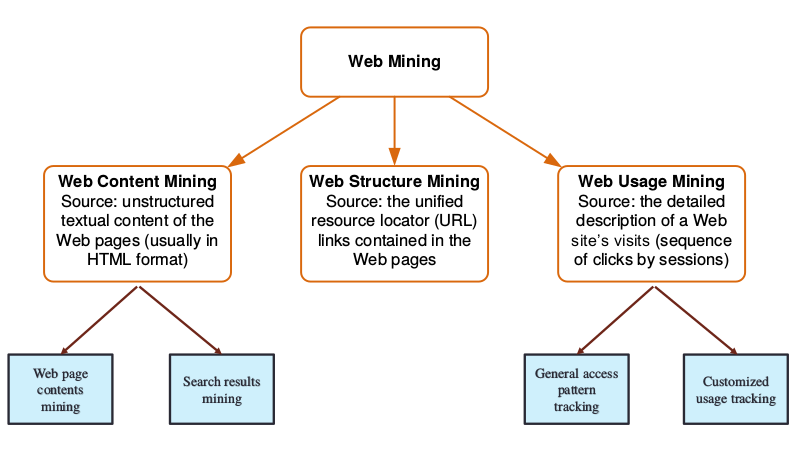
\includegraphics[width=0.7\textwidth]{figures/typed-of-webmining.png}
%    \caption{dummy}
%    \label{fig:XXX}
%\end{figure}

\subsubsection{Ethical considerations}
How do we store the data? What is the problem with Google forms. (Maybe write that in a real research we would use our own form/tool!)

\subsubsection{Legal considerations}
GDPR checkbox in the survery

\subsubsection{Applied tools}
About google forms and R, maybe

\section{Analysis}

\subsection{Pilot}

\subsection{Absolute and Relative Frequencies}

\subsection{(Co-)variances}

\subsection{Independence}

\section{Conclusion}

\section*{References}
\bibliographystyle{ieeetr}
\renewcommand\refname{\vskip -1cm}
\bibliography{ST3012_project_report_v19pette_v18tobwe}

\section*{Appendices}

\subsection*{Survey Guideline}
Information about the questions

\subsection*{Survey Questions}
Only absolute relevant questions

\subsection*{DESAP checklist}
Checklist can be found in the git folder

\end{document}
